
\newrefcontext[sorting=ynt]

\lettrine{T}{ropical} montane ecosystems are hotspots of biological diversity and are home to over 70\% of the world's avian diversity in less than 10\% of global terrestrial area \citep{myers2000,davies2007,quintero2018}.
However, tropical mountains are under tremendous anthropogenic pressures of habitat modification and climate change, which can both have negative consequences for bird species \citep{nogues-bravo2007,newbold2015}.
In addition to directly affecting bird populations, climate change and changes in land cover can also affect species distributions in montane areas worldwide \citep{nogues-bravo2007,rahbek2019}.
For example, mountain birds in California tracked changes in temperature and precipitation over a century of climate change, illustrating the long-term role of climate in driving range shifts \citep{tingley2009}.
The movement of temperature bands upslope can eliminate the conditions to which high-altitude species are adapted, leading to local extinction \citep{freeman2018,urban2018}.
A combination of changes in climate and land cover best explains the colonization and extinction probabilities of North American birds \cite{yalcin2018}.
However, few studies have disentangled the role of these two drivers on species' current distributions \citep{sirami2017}.
Furthermore, species distributions in tropical mountains especially are poorly studied despite being `escalators to extinction' for montane birds \citep{elsen2017,freeman2018,srinivasan2019,srinivasan2021}.
Understanding the contemporary drivers of species' distributions in tropical mountains can help predict future species ranges as the climate changes \citep{guo2018,srinivasan2021}.

The drivers of bird distributions in tropical montane ecosystems are poorly understood because data on species distributions in these regions are limited \citep{payne2017,peters2019}.
Citizen science efforts offer a solution: initiatives such as \textit{eBird} are growing in popularity and scale and make the observation data readily available to researchers \citep{sullivan2014}.
\textit{eBird} combines many thousands of decentralized, ad hoc, organized, or semi-organized bird observations to form representative samples of species' occurrence over vast scales \citep{sullivan2009,sullivan2014,wood2011a}.
The standardization of the reporting infrastructure (e.g., the \textit{eBird} mobile app or website) allows observations to be reproducibly processed to achieve a high standard of reliability.
For example, one can filter out short observation sessions that might not accurately capture a location's bird community or weight observations by the observer's effort \citep{kelling2015a,johnston2018,johnston2021}.
Including data from citizen scientist observations can significantly improve species distribution models \citep{robinson2020}, and enable a wide range of research, including mapping species elevational movements \citep{tsai2020} and prioritizing conservation efforts \citep{vanstrien2013,fink2014,johnston2015}.
India reports one of the largest numbers of \textit{eBird} checklists from a tropical country, as birdwatchers have contributed to \textit{eBird} in a concerted and growing effort since 2014 \citep{viswanathan2020}.
Coordinated citizen science efforts have led to successfully mapping the distribution and abundance of birds across multiple regions in India \citep[e.g. the Mysore Bird Atlas, and the Kerala Bird Atlas][]{praveenj2021}.
As of March 2021, the \textit{eBird} India dataset has grown to a total of over 14 million observations across 1,342 species of birds.

We set out to examine the role of climate and land cover and its association with bird occupancy in a tropical montane region, the Western Ghats of southern India.
The Western Ghats mountain ecosystem is part of the Western Ghats-Sri Lanka biodiversity hotspot and is home to numerous species of endemic plants and animals \citep{myers2000,das2006}.
We examined observations from \textit{eBird} between 2013 and 2021 for 79 species (later reduced to 55, following model fitting) of birds across the two largest hill ranges in the southern Western Ghats --- the Nilgiri and the Anamalai-Palani hills (see Fig.~\ref{hilly_fig_01}a).
Specifically, we tested associations between climatic variables, land cover, and bird occupancy.
We binned species according to their habitat preference prior to hypothesis testing; a species could either be a forest species (species found in forested/woodland habitats as well as forest edges) or generalist species (widespread species found across a range of habitat types) \citep{ali1983}.

First, we examined the direction of association between species-specific probability of occupancy and climatic predictors.
Temperature seasonality: We tested the hypothesis that the probability of occupancy of forest specialist birds should be negatively associated with temperature seasonality (coefficient of variation) \citep{srinivasan2018}.
Tropical forest species are often associated with a narrow range of temperatures leading to the expectation that the probability of occupancy will decrease with increasing variation in temperatures \citep{janzen1967,stevens1989,frishkoff2016,chan2016,srinivasan2018}.
However, we expected that the occupancy of generalist species may be positively associated with temperature seasonality.
In other words, we expected that generalist species have broader thermal niches and occur in climatically variable regions when compared to their forest counterparts.
Precipitation seasonality: the `hygric' niche hypothesis states that species often occur within an optimal range of rainfall conditions \citep{boyle2020}.
Across our study area, we expected that precipitation seasonality (coefficient of variation) would be positively associated with species occupancy for forest birds and negatively associated with generalist bird species.
Forest species in the Western Ghats are largely seen in wetter habitats relative to generalist species that are more often found in drier habitats \citep{raman2006}.
Finally, we examined the direction of association between species-specific probability of occupancy and land cover.
We expected the occupancy of forest species to be positively associated with naturally occurring land cover types such as evergreen forests and deciduous forests.
We expected that human-modified land cover types, including agriculture, settlements, and plantations would be positively associated with species-specific probability of occupancy of generalist birds.

\subsection*{Methods}

\subsubsection*{The Southern Western Ghats}

The Nilgiri and the Anamalai-Palani hills (hereafter, Anamalai hills) (Fig.~\ref{hilly_fig_01}) are part of the Western Ghats, an ancient region of differentiation of flora and fauna in South Asia \citep{mani1974,myers2000,vijayakumar2016}.
These hill ranges host a diversity of land cover types, possess a wide climatic gradient, and several bird species \citep{ali1983,das2006}.
The elevational range across these hill ranges varies from 40m in the plains to 2,625m in the higher elevations.
(Fig.~\ref{hilly_fig_01}a).
These two hill ranges are home to a multitude of habitats, ranging from high elevation grasslands (>1400m; Fig.~\ref{hilly_fig_01}b) to mid-elevation evergreen forests (>700m and <1400m; Fig.~\ref{hilly_fig_01}b).
These hill ranges interact strongly with the annual south-west monsoon resulting in orographic rainfall on the western slopes ($\sim$3000 mm) and a relative rain-shadow on the leeward eastern slopes ($\sim$2000 mm) that in turn influences the distribution of endemic flora and fauna \citep{gadgil1986,pascal1988,robin2015}.

\begin{figure}[h!]
    \centering
    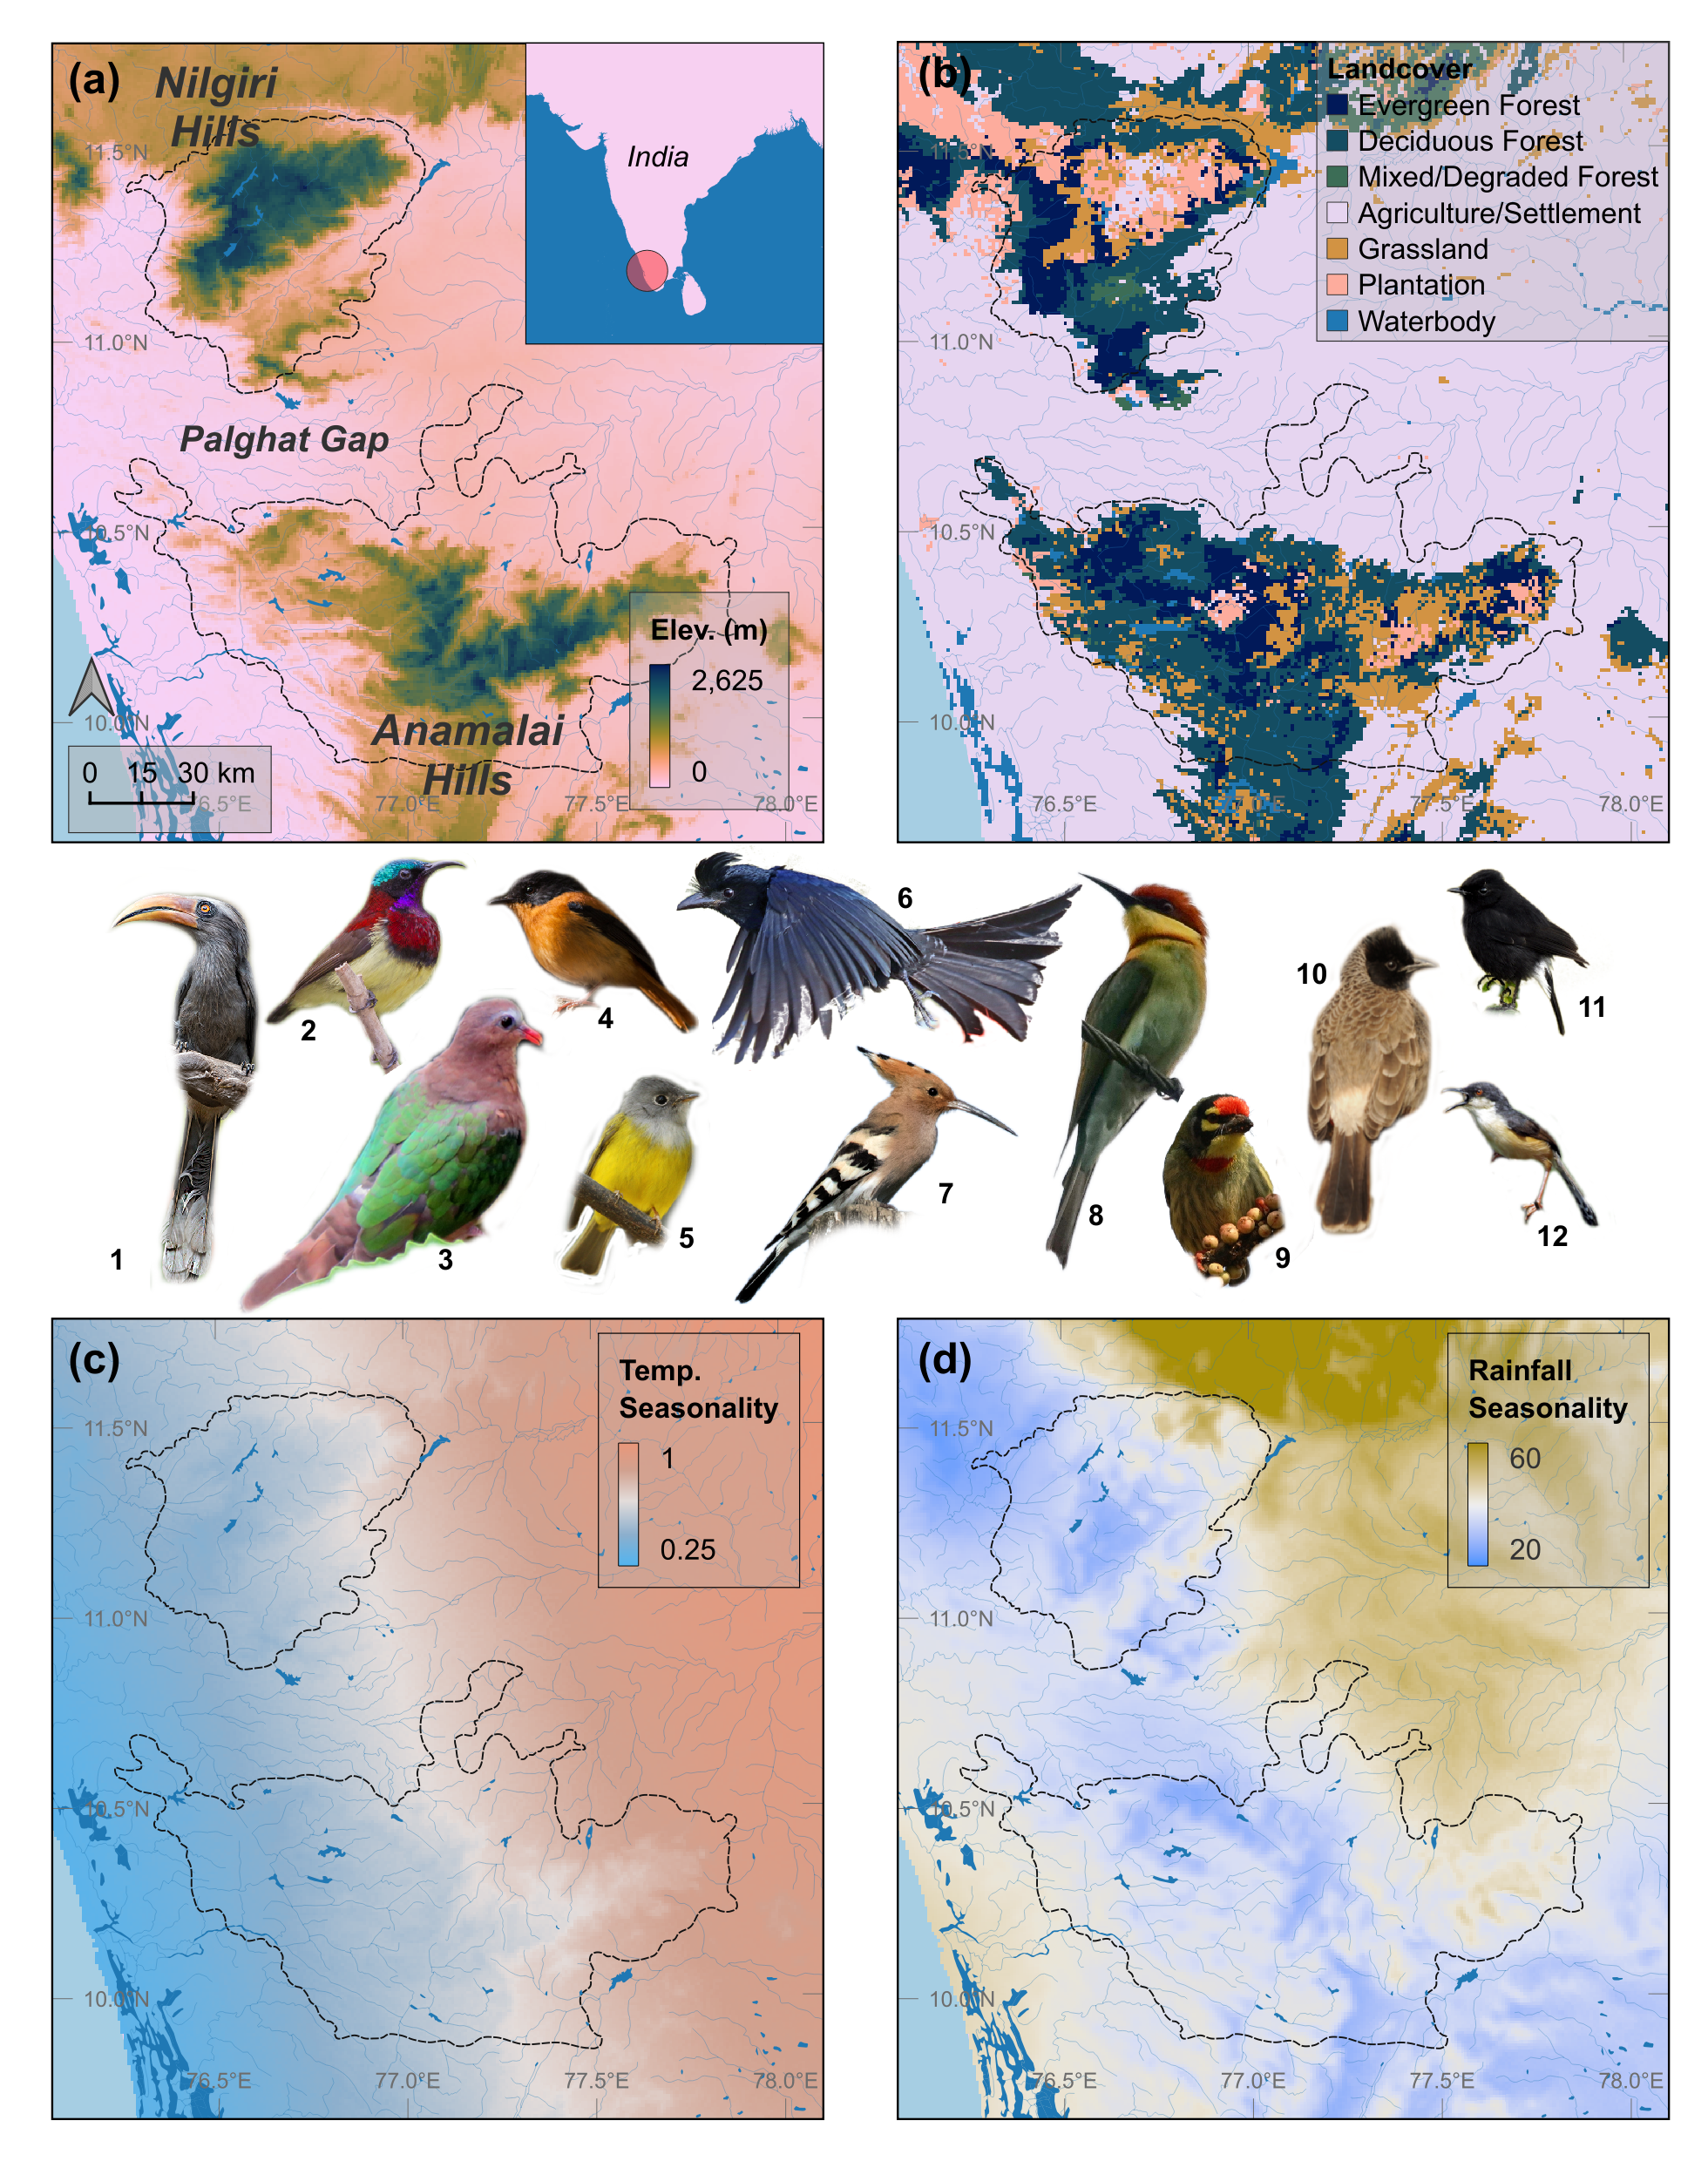
\includegraphics[width=0.9\textwidth]{figures/hillybirds/fig_01.png}
    \caption{
        \textbf{The Nilgiri and Anamalai Hills in southern India provide a convenient geography for studying the interplay of land cover and climate on the distributions of bird species.}
        \textbf{(a)} The Nilgiri and Anamalai Hills of the Southern Western Ghats are topographically complex, with maximum elevations > 2,000 m, and are separated by the very low-lying Palghat Gap, which serves as a natural barrier to the dispersal of many hill birds. 
        \textbf{(b)} Lower elevations are primarily covered by agriculture and settlements, reflecting the intense human pressure on this region, while mid- and higher elevations show a mix of natural and human-modified land cover types (see Fig.~\ref{hilly_fig_02} for details). 
        \textbf{(c)} The coastal edge of the area, and the windward hill slopes show limited temperature seasonality across the December -- May period; this seasonality increases with distance from the coast but is lower at higher elevations inland. 
        \textbf{(d)} Higher elevations also show limited precipitation seasonality than both low-lying coastal and inland regions. 
        Our study area (bounds shown as dashed lines) includes multiple combinations of elevation, land cover type, and temperature and rainfall seasonality, resulting in a naturally occurring crossed-factorial design that allows us to study the effects of climate and land cover on bird occupancy. 
        Representative forest-restricted and habitat-generalist birds from the study area are shown between panels (all images were obtained from Wikimedia commons and credit is assigned for each species in brackets).
        % ; From L to R: (1) Malabar grey hornbill (by Koshy), (2) Crimson-backed sunbird (by Mandar Godbole), (3) Asian emerald dove (by Selvaganesh), (4) Black-and-orange flycatcher (by LKanth), (5) Grey-headed canary flycatcher (by David Raju), (6) Greater-racket tailed drongo (by MD Shahanshah Bappy), (7) Eurasian hoopoe (by Zeynel cebeci), (8) Chestnut-headed bee-eater (by Mik\textit{eBird}s), (9) Coppersmith barbet (by Raju Kasambe), (10) Red-vented bulbul (by TR Shankar Raman), (11) Pied bushchat (by TR Shankar Raman), (12) Ashy prinia (by Rison Thumboor). 
        Elevation is from 30m resolution SRTM data (Farr et al. 2007), land cover, at 1km resolution, is reclassified from Roy et al. (2015), while climatic variation is represented by CHELSA seasonality layers (temperature: BIOCLIM 4a, rainfall: BIOCLIM 15), at 1km resolution (Karger et al. 2017). All layers were resampled to 1km resolution for analyses.
    }
    \label{hilly_fig_01}
\end{figure}

\begin{figure}[h!]
    \centering
    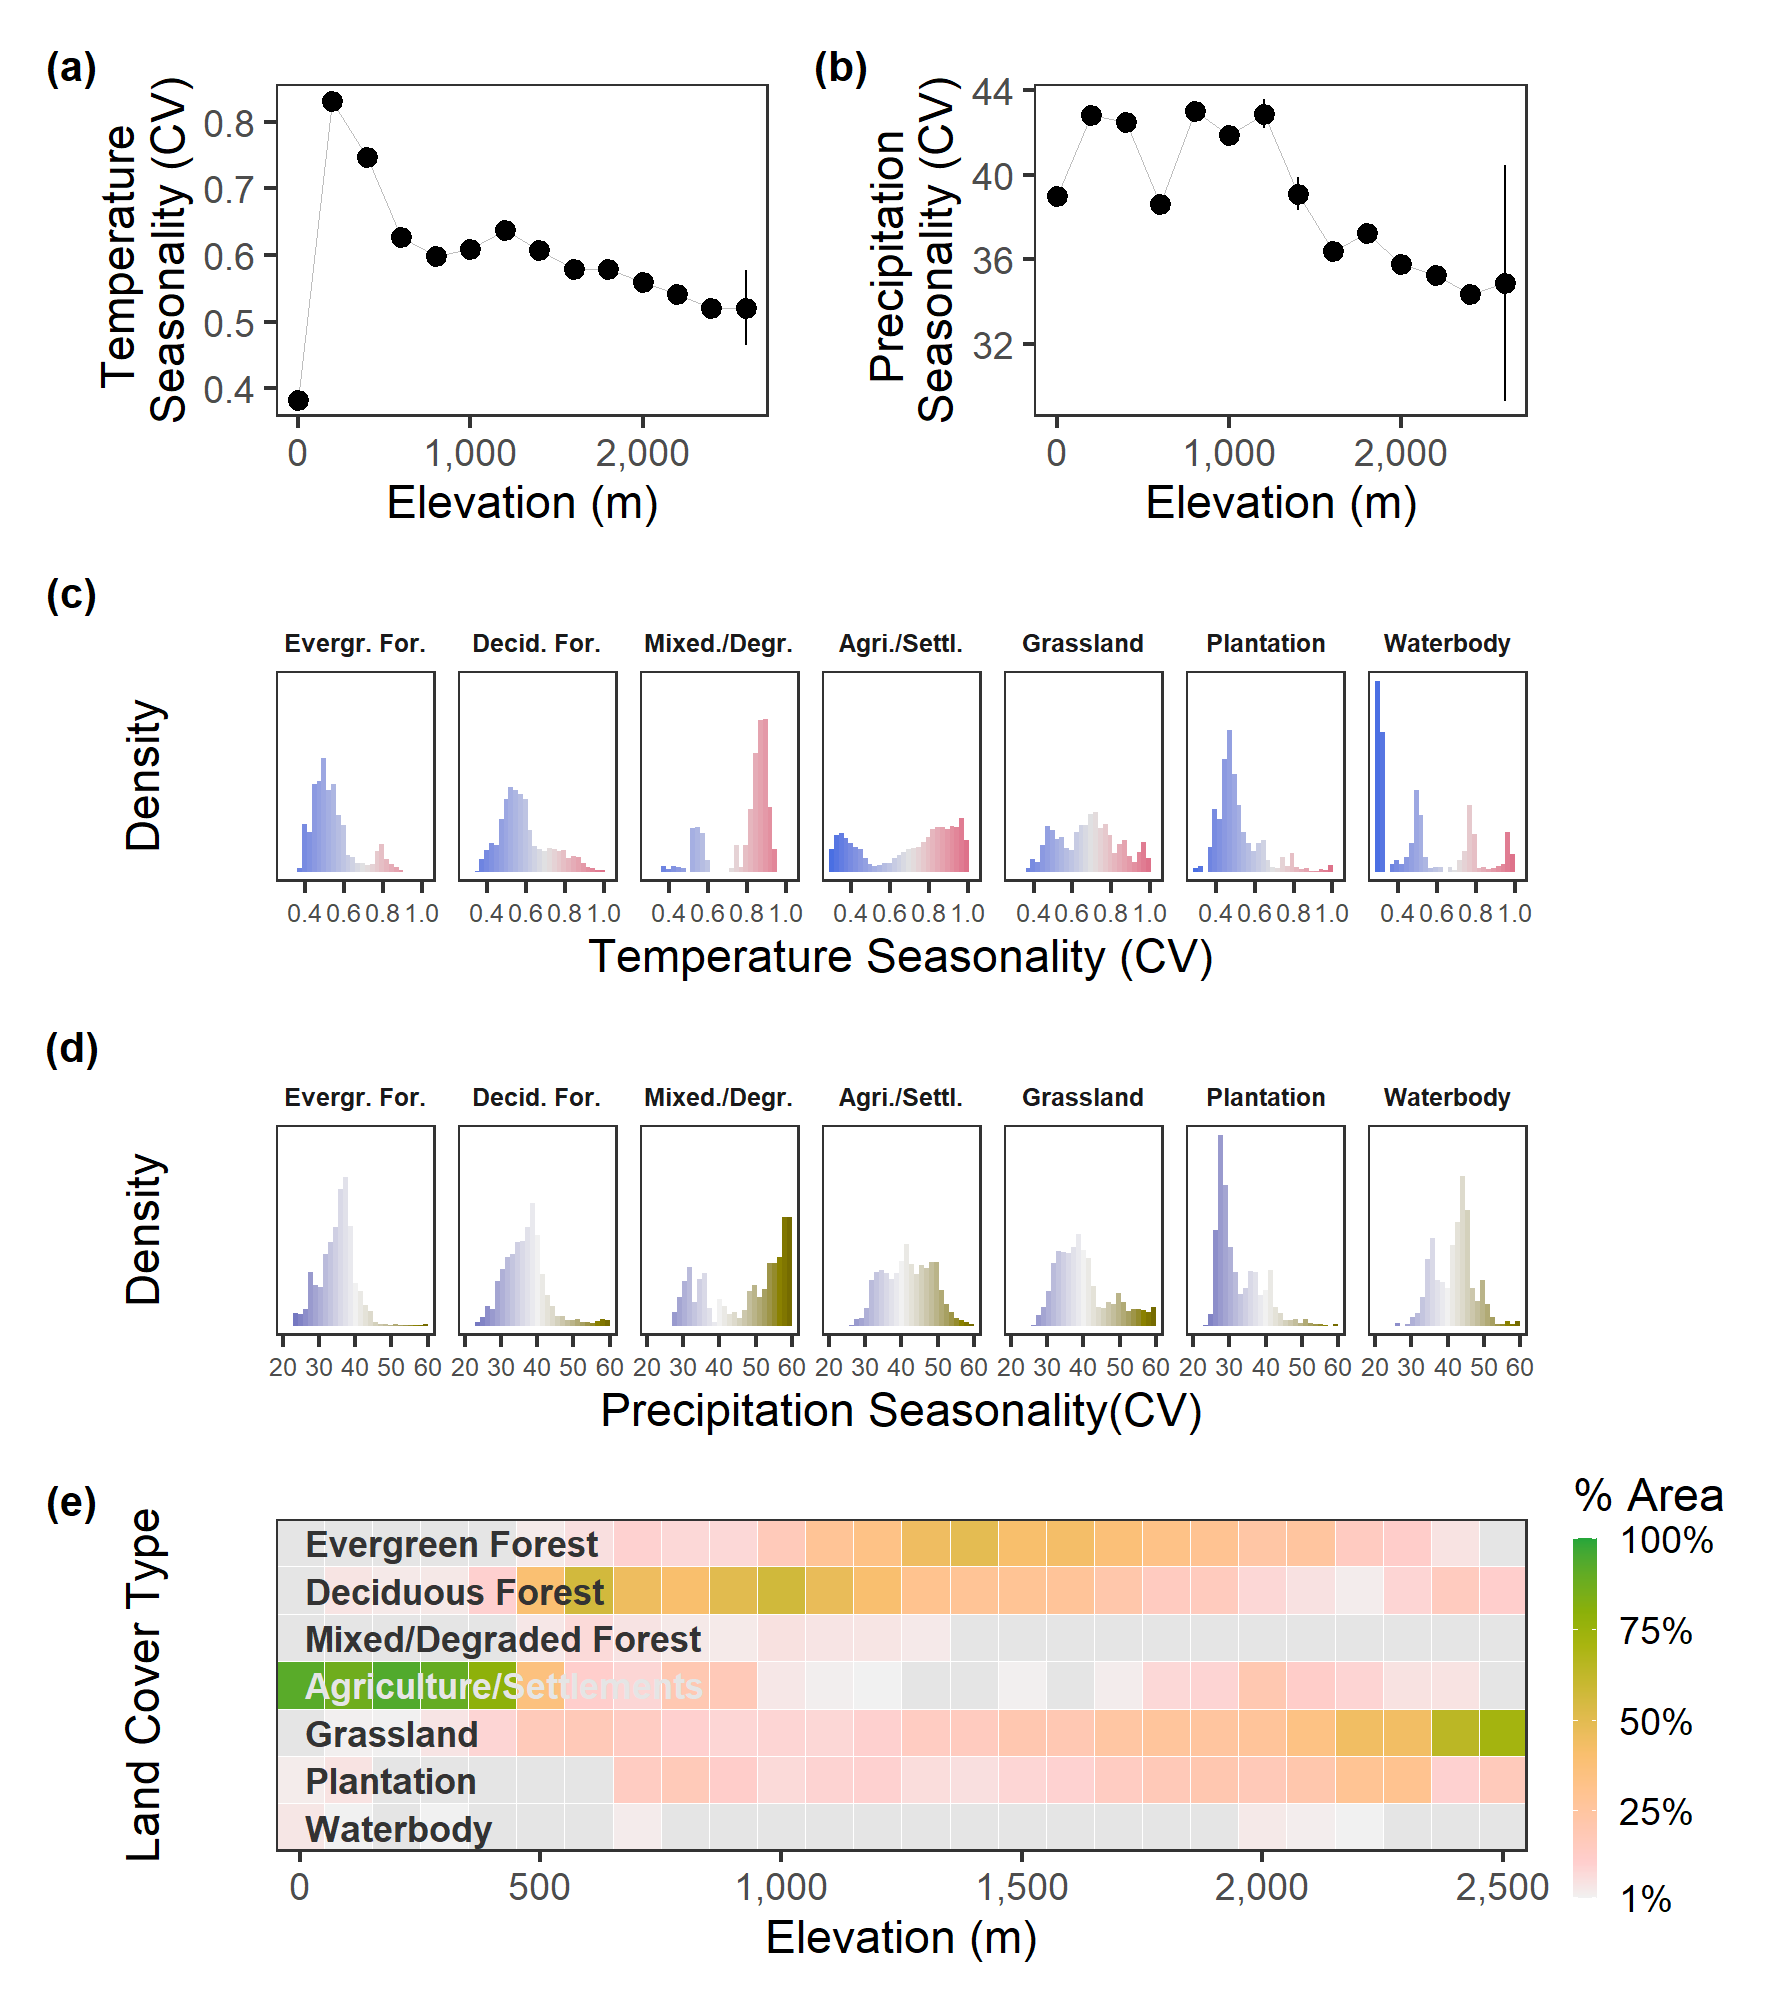
\includegraphics[width=0.9\textwidth]{figures/hillybirds/fig_02.png}
    \caption{
        \textbf{Climate and land cover vary strongly along the elevation gradient in the Nilgiri and Anamalai Hills.}
        Both \textbf{(a)} temperature seasonality and \textbf{(b)} precipitation seasonality, between the months of December and May, declines with increasing elevation across the Nilgiri and Anamalai Hills. 
        Climatic variation is not very strongly associated with land cover type, as both natural habitats such as forests, and human-associated habitat types such as plantations show low seasonality in \textbf{(c)} temperature, and \textbf{(d)} precipitation.
        \textbf{(e)} Most elevations host a range of land cover types: while human-associated habitats such as agriculture are concentrated at lower elevations, and more natural types such as grasslands and forests are associated with higher elevations, each of these types is also found outside their characteristic elevational bands.
        We calculated climate seasonalities (BIOCLIM 4a and 15: temperature and precipitation, respectively) using CHELSA data over 1979 -- 2013, from December to May (Karger et al, 2017), and present mean seasonality values (vertical bars show standard deviation) for every 200m elevational band
        Land cover types were taken from a reclassification of Roy et al
        (2015; see main text) at 100m elevational bands.
        Land cover types covering < 1\% of an elevational band are shaded grey
        All landscape layers were first resampled to 1km resolution.
    }
    \label{hilly_fig_02}
\end{figure}

\subsubsection*{Filtering \textit{eBird} Data}

Data from \textit{eBird} is available in the form of a `checklist' submitted by an observer or a group of observers.
Each checklist includes a wide range of information that includes species identity, latitude, longitude, date of observation, distance traveled, time spent observing etc.
`Complete' checklists indicate that the observer(s) recorded all the birds detected and identified.
We obtained bird detections from such complete checklists contributed to \textit{eBird} for nine years (2013 to 2021) across the Nilgiri and Anamalai hill ranges.
Only checklists recorded during December to May (non-rainy months) were included in our study because detecting birds during the rainy months is difficult due to poor weather.
Restricting our data to complete checklists also allowed us to interpret the absence of a species on a checklist as a non-detection \citep[called zero-filling][]{johnston2021}.
Even when restricting analysis to only `complete' checklists, the semi-structured, flexible nature of databases like \textit{eBird} results in large variation in effort across checklists as a result of the often opportunistic nature of data collection \citep{kelling2019}.
Complete checklists are marked as `Stationary' or `Traveling' based on the distance traveled by an observer while recording detections.
To reduce variation in observer effort, we first considered only those complete checklists with a duration ≤ 300 mins (5 hrs), and distance ≤ 5km (for traveling checklists), and with fewer than 10 observers \citep[following][]{johnston2019}.
Since stationary birdwatchers can detect birds up to 100m away, we set all stationary checklists to a distance of 100 m.
In many cases, checklists are submitted by a single observer for a group of birdwatchers; in such cases, the group checklist only occurs once in the dataset.
We used only checklists recorded between 5:00 AM and 7:00 PM to avoid sightings in low-light conditions.

\subsubsection*{Selecting Study Species}

We limited our study to 79 species of terrestrial, diurnal birds that occur in our study region (see list of species in {\color{red}Appendix S1}; see Fig.~\ref{hilly_fig_01} for representative species).
We selected these species using inclusion criteria adapted from the State of India's Birds Report 2020 \citep[SoIB][]{viswanathan2020}.
We intended these criteria to ensure uniform sampling of each species across our study area, and to reduce erroneous associations between environmental drivers and species distributions.
Beginning with 3.37 million observations of 684 species in \textit{eBird} that occurred within the outlines of our study area (Fig.~\ref{hilly_fig_01}a), over the years 2013 -- 2021, we retained only those species that had a minimum of 1,000 detections each between 2013 and 2021 (347 species remaining; 3.33 million observations).
Next, we divided the study area into 25 $\times$ 25km grid cells (42 unique cells; see supplementary material).
We kept only those species that occurred in at least 5\% of all checklists across at least 27 unique grid cells (50\% of the study area).
We further manually removed raptors (\textit{Accipitriformes} and \textit{Falconidae}), swifts (\textit{Apodiformes}), and swallows (\textit{Hirundinidae}) since these birds are usually observed in flight when species identification can be prone to errors.
This filtering process resulted in a total of 1.29 million observations (presences) across our study area.

\subsubsection*{Spatio-temporal bias in occurrence data}

Sampling bias can be introduced into citizen science observations due to the often opportunistic nature of data collection \citep{sullivan2014}.
For \textit{eBird}, this translates into checklists reported when convenient, rather than at regular or random points in time and space, leading to non-independence in the data if observations are spatio-temporally clustered \citep{johnston2021}.
For example, sites near roads are easier to reach and maybe sampled more frequently.
The spatial clustering of observations can be reduced by sub-sampling at an appropriate spatial resolution \citep{aiello-lammens2015}; however, thinning the data over-zealously can result in very few presence records compared to absence records \citep[i.e., class imbalance][]{steen2019}.
Consequently, when there are many more absence records than presence records, presences and absences should be handled separately when spatially thinning the data.

We first estimated two simple measures of spatial clustering: the distance from each site to the nearest road \citep[road data from OpenStreetMap:][]{openstreetmapcontributors2017} and the nearest-neighbor distance for each site.
Sites were strongly tied to roads (see Fig.~\ref{hilly_fig_03}a.; mean distance to road $\pmin$ SD = 390.77 $\pmin$ 859.15m; range = 0.28m -- 7.64km) and were on average only 297m away from another site (SD = 553m; range = 0.14m -- 12.85km).
This is understandable, as roads and trails provide access, and particular well-known areas are visited often.
On average, across species, presences comprised only 8.5\% of all observations.
We followed \textcite{steen2021} in choosing to spatio-temporally thin only the absences, and not the presences, for each species --- a methodology called `thin majority' that can improve model performance \citep{steen2021}.
To do this, we divided the study area into a grid of 500m wide square cells, and from within each cell, we chose the site with the most visits (checklists) over the sampling period.
From each of the remaining sites, we selected a maximum of 10 random absence checklists to reduce temporal clustering, keeping all absence checklists for sites with ≤ 10 checklists.
We retained all presences for each species without any spatial or temporal thinning \citep{steen2021}.
As a result of class balancing, in our final dataset, presences made up 29.3\% of observations on average across species.

\begin{figure}[h!]
    \centering
    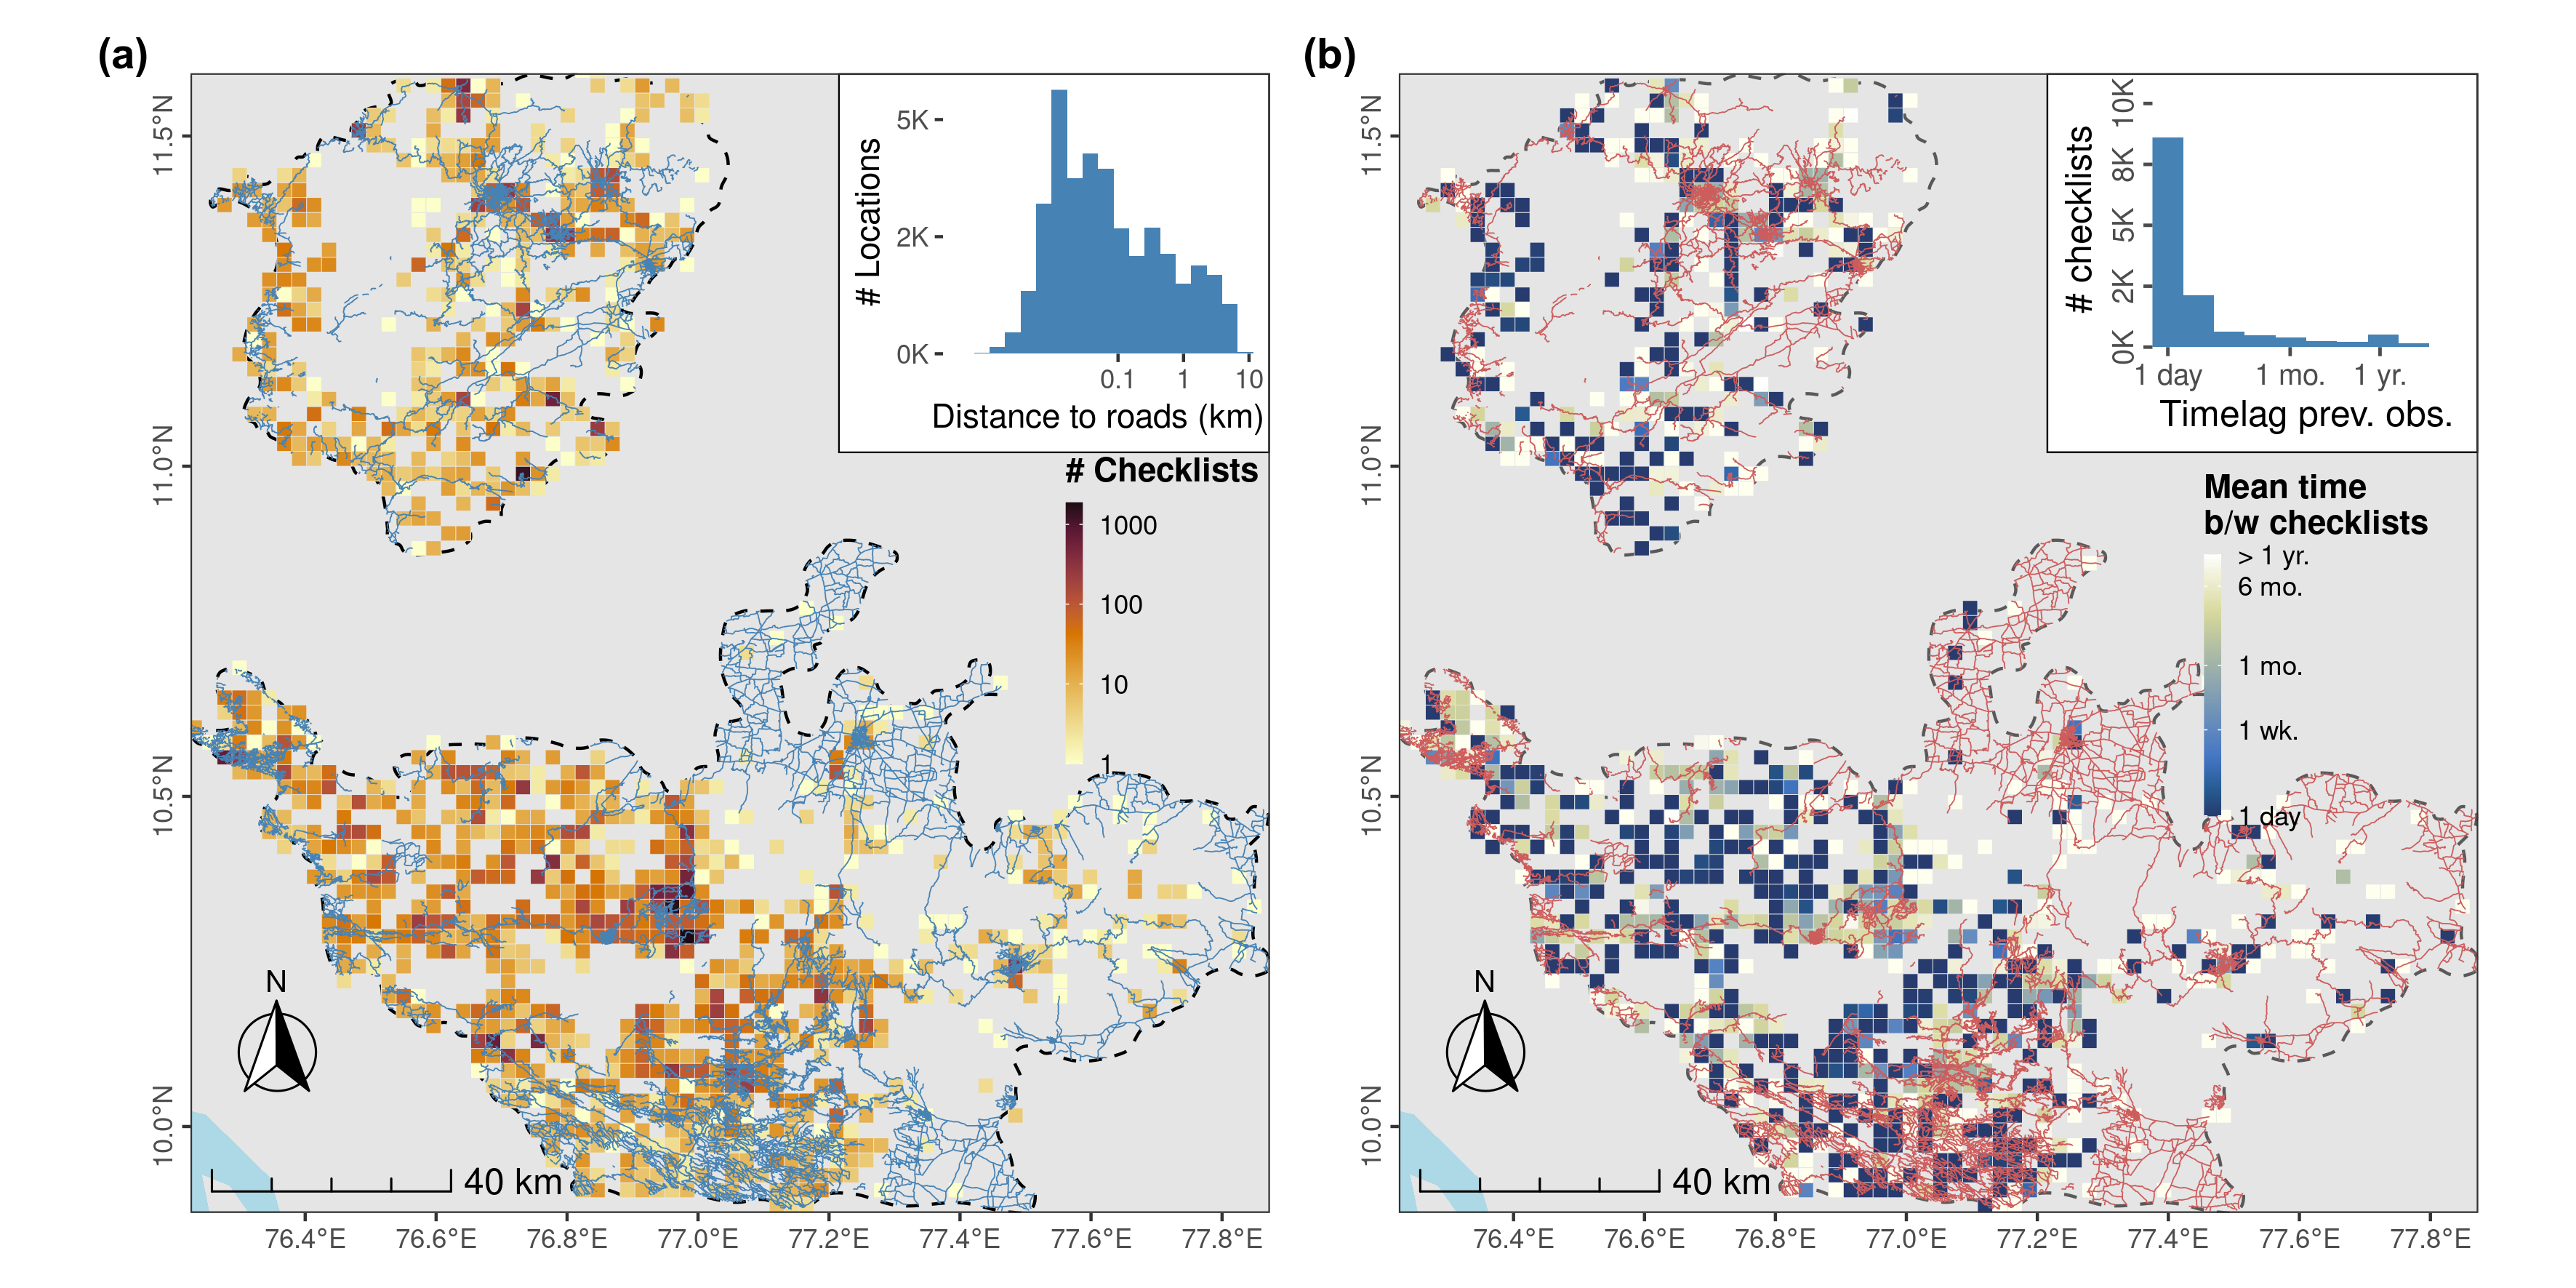
\includegraphics[width=0.9\textwidth]{figures/hillybirds/fig_03.png}
    \caption{
        \textbf{Distribution of sampling effort in the form of \textit{eBird} checklists in the Nilgiri and Anamalai Hills between 2013 and 2021.}
        \textbf{(a)} Sampling effort across the Nilgiri and Anamalai Hills, in the form of \textit{eBird} checklists reported by birdwatchers, mostly takes place along roads, with the majority of checklists located $<$ 1km from a roadway (see distribution in inset), and therefore, only about 300m, on average, from the location of another checklist.
        \textbf{(b)} \textit{eBird} checklists are also strongly clustered in time, with some of the most sampled areas over the study period visited at intervals of $>$ 1 week, and with some less intensively sampled areas visited frequently, at intervals of $<$ 1 week.
        Overall, most checklists are reported only a day after the previous checklist at that location (see inset).
        Both spatial and temporal clustering make data thinning necessary.
        Both panels show counts or mean intervals in a 2.5km grid cell; the study area is bounded by a dashed line, and roads within it are shown as (a) blue or (b) red lines.
    }
    \label{hilly_fig_03}
\end{figure}

\subsubsection*{Adjusting for Spatial Precision}

Every checklist on \textit{eBird} is associated with a latitude and longitude.
However, the coordinates entered by an observer may not accurately depict the location at which a species is detected.
Such an error can occur for two reasons: first, traveling checklists are associated with a single location along the route travelled by observers.
Second, checklist locations could be assigned to a `hotspot' --- a location that is automatically marked by \textit{eBird} as being frequented by multiple observers --- even though the observation was not made at the precise location of the hotspot \citep{praveenj.2017}.
Since a large proportion of observations occur within 3km of the observation effort's starting point, we adjusted for the spatial precision of \textit{eBird} records by considering a buffer radius of 2.5km around each site when sampling environmental covariate values.

\subsubsection*{Calibrating Observations Across Observers}

Differences in bird identification skills among citizen scientists can lead to biased species detection when compared with data collected by a consistent set of trained observers \citep{vanstrien2013}.
Including observer calibration (that accounts for observer-specific differences in identification) as a detection covariate in occupancy models using \textit{eBird} data can help account for this variation \citep{johnston2018}.
Observer-specific calibration in local avifauna was calculated following \textcite{kelling2015a} as the normalized predicted number of species reported by an observer after 60 minutes of sampling across the most common land cover type within the study area (in our case, deciduous forests).
This score was calculated by examining checklists from anonymized observers across the study area.
We modified the \citep{kelling2015a} formulation by including only observations of the 79 species of interest in our calculations.
An observer with a higher number of species of interest reported within 60 minutes would have a higher observer-specific calibration score, with respect to the study area.
We then estimated a checklist calibration index (CCI) from observer-specific calibration scores associated with each checklist.
The CCI was the lone observer's calibration score for single-observer checklists and the highest calibration score among observers for group checklists.
CCI is predicted from a generalized linear mixed effects model:
\begin{multline*}
    \text{n} \sim \text{duration} + \sqrt{\text{duration}} + \text{landcover} + \sqrt{\text{time of day}} + \sqrt{\text{time of day}}^2 + \\ \log({\text{julian date})} + \log({\text{julian date})}^2 + (1 | \text{observer}) + \\(0 + \text{duration} | \text{observer})
\end{multline*}
where, $n$ is the number of species observed in that checklist, \textit{duration} is the time spent observing birds for the checklist, \textit{landcover} refers to the land cover type, \textit{time\_of\_day} refers to the time of the day that observations were made, and \textit{julian\_date} refers to the ordinal day of the year.

\subsubsection*{Preparing Occupancy Predictors}

We prepared a suite of climatic and land cover variables to be modeled as covariates of species-specific probabilities of occupancy within our full study region (Figs.~\ref{hilly_fig_01} -- \ref{hilly_fig_02}).
Among climatic predictors, we chose to examine the effects of temperature and precipitation seasonality on species occupancy, and we obtained these predictors at a spatial scale of 1km \citep[Climatologies at High resolution for the Earth's Land Surface Areas; CHELSA:][]{karger2017}.
Temperature seasonality is defined as the amount of temperature variation over a given time period based on the ratio of the standard deviation of the monthly mean temperatures to the mean of the monthly temperatures \citep{odonnell2012}.
In other words, temperature seasonality is the coefficient of variation and captures the dispersion in relative terms because standard deviation can produce two similar values while the means may be different.
Larger values of temperature seasonality imply higher variability in temperature, relative to the average temperature.
It is important to calculate variability relative to the mean because the same amount of statistical variability (e.g., variance) in a dry area as a wet area would have a much bigger `seasonality' impact on a dry area.
Similarly, we defined precipitation seasonality as the ratio of the standard deviation of the monthly total precipitation to the mean monthly total precipitation \citep{odonnell2012}.
The above calculations of seasonality were made using temperature and precipitation data from CHELSA for the non-monsoon months of December to May for our study area.
While data from global databases such as WorldClim have been used for modeling species distributions, CHELSA data has shown greater predictive power \citep{karger2017} and hence we used the latter in this study.
Other bioclimatic predictors such as mean annual temperature, mean annual precipitation, mean temperature of the coldest or driest quarter, or the precipitation of driest or coldest quarter were equally well suited for our study; however, they were highly correlated ($|r|$ $>$ 0.5) with temperature and precipitation seasonality.
We obtained land cover over our study site from a high-resolution vegetation type map generated by \citep{roy2015}, using medium resolution IRS-LISS III (Indian Remote Sensing Satellite - Linear Imaging Self Scanner) images (http://bis.iirs.gov.in/).
This classification was originally generated at a scale of $\sim$23m and with 22 land cover classes for our study area.
We aggregated these 22 classes into seven broad, ecologically relevant land cover types: evergreen forests, deciduous forests, mixed/degraded forests, agriculture/settlements, plantations, grasslands, and water bodies (see Supplementary Material).
We resampled the reclassified land cover layer using a nearest neighborhood approach to 1km to match the 1km resolution of the climatic layers.

Testing for collinearity among the climatic and land cover predictors did not result in the removal of any predictors as the correlations were low ($|r| <$ 0.5).
We then pooled the climatic (n = 2) and land cover (n = 7) predictors and calculated mean values for the two climatic predictors (temperature seasonality and precipitation seasonality) and calculated the proportion of each of the seven land cover types within the 2.5km buffer radius around each spatio-temporally thinned locality for each species.

\subsubsection*{Estimating Species Occupancy}

Occupancy models estimate the probability of occurrence of a given species while controlling for imperfect detection and allow us to model the factors affecting occurrence and detection independently \citep{mackenzie2017,johnston2018}.
The flexible \textit{eBird} observation process contributes to the largest source of variation in the likelihood of detecting a particular species \citep{johnston2021}; hence, we included six continuous covariates that influence the probability of detection for each checklist: ordinal day of year, duration of observation, distance travelled, time of day of observations, number of observers, and the checklist calibration index (CCI).
We converted calendar date into a linear, continuous predictor by extracting ordinal days of the year (julian date) for December to May and scaling them between 1 and 183 (dates in December subtracted from 333, and 31 added to dates between January and May).
This time period essentially includes winter and summer seasons (loosely defined) in the Western Ghats where detectability of bird species is high.
Our breeding season is often toward the end of this window (late April to early May) when resident species begin to breed while migratory birds travel back to their breeding grounds.
We modeled time of day so as to allow detectability to be highest at dawn and dusk when birds often sing and are easily detected, and to be lower in the middle of the day, when birds are least active and thus less likely to be detected.

Using a multi-model information-theoretic approach, we tested how strongly our occurrence data fit our candidate set of environmental covariates \citep{burnham2002}.
We fitted single-species occupancy models for each species, to simultaneously estimate a probability of detection ($p$) and a probability of occupancy ($\psi$) \citep{mackenzie2002,fiske2011}.
For each species, we fit 512 models, each with a unique combination of the (climate and land cover) occupancy covariates and all detection covariates (the six detection covariates are present in every model).

\begin{multline*}
    \text{logit}(p) \sim \text{julian date} + \text{duration} + \text{distance} + \text{obs. started} + \\
    \text{number observers} + CCI    
\end{multline*}

where \textit{julian date} refers to the ordinal day of the year, \textit{duration} refers to the time spent observing birds in minutes, \textit{distance} is the distance travelled by the observer(s) in kilometers, \textit{obs. started} is the time of day when observations were recorded, \textit{number observers} refer to the number of observers, and $CCI$ is the checklist calibration index.

\begin{multline*}
    \text{logit}(\psi) \sim \text{BIO 4a} + \text{BIO 15} + p(\text{Evergreen}) + p(\text{Deciduous}) + \\
    p(\text{MixedDegraded}) + p(\text{AgricultureSettlements}) + p(\text{Plantations}) + \\
    p(\text{Grasslands}) + p(\text{WaterBodies})
\end{multline*}

Previously, we explored the non-linear effects of temperature seasonality and precipitation seasonality.
However, our occupancy models showed a poor fit to the data when temperature and precipitation seasonality were included as non-linear terms and hence, we did not explore this further.
Adequate model fit was assessed using a chi-square goodness-of-fit test using 1,000 parametric bootstrap simulations on a global model that included all occupancy and detection covariates (MacKenzie and Bailey 2004).
Across the 512 models tested for each species, the model with highest support was determined using AICc scores.
However, across the majority of the species, no single model had overwhelming support.
Hence, for each species, we examined those top models which had a difference in AICc of $<$ 4, as these top models were considered to explain a large proportion of the association between the species-specific probability of occupancy and environmental drivers \citep{burnham2011}.
Using these restricted model sets for each species; we created a model-averaged coefficient estimate for each predictor and assessed its direction and significance \citep{barton2009}.
These model-averaged coefficients include zeros when a predictor is absent in one of the top models.
In addition, we estimated a model-averaged standard error using which we calculated a 95\% confidence interval \citep{burnham2002}.
We considered a predictor to be significantly associated with occupancy if the range of the 95\% confidence interval around the model-averaged coefficient did not contain zero.

Prior to further inference, all 79 birds in our study were classified as forest species or generalist species following \citep{ali1983}.
Forest species are those that are typically found in wet evergreen, semi-evergreen, deciduous, moist deciduous forests, and other woodland habitats as well as forest edges.
This classification encompasses specialist endemic birds, species that occur in woodland habitats as well as those species found along the edges of forested areas.
Generalist species are those that are typically found across a range of habitat types such as forests, agricultural lands, settlements, etc.

All continuous covariates were standardized prior to analysis, allowing for the comparison of model-averaged coefficients between species.
We used the R packages unmarked, and MuMIn for occupancy modeling and model averaging; the code provided in the supplementary material and on our Github repository shows the full set of R and Python packages used in this work \citep{barton2009,fiske2011,r2020}.

\subsubsection*{Data deposition}

All data were downloaded from \textit{eBird} (version 1.13) and can be accessed via: http://\textit{eBird}.org/data/download.
The complete analysis is available as Supplementary Material (https://github.com/vjjan91/\textit{eBird}Occupancy) and is archived on Zenodo (https://doi.org/10.5281/zenodo.6025640).

\section*{Results}

Following spatio-temporal thinning of observations, we relied on 315,428 curated citizen scientist observations (including both presences and non-detections) across 79 species of birds between 2013 and 2021 for modeling occupancy.
The number of detections varied from a minimum of 224 observations to a maximum of 7,725 observations per species (following spatio-temporal thinning).
Chi-square goodness-of-fit tests suggested a poor model fit for twenty-four species ($p <$ 0.05; Appendix S2) and hence these species were removed before further analysis (resulting in a total of 55 species).
Of the list of 55 species, six species were migratory species (long-distance/altitudinal) that are present in our study area during the focal seasonal time period: Blyth's reed warbler \textit{Acrocephalus dumetorum}, Brown shrike \textit{Lanius cristatus}, Chestnut-headed bee-eater \textit{Merops leschenaulti}, Grey wagtail \textit{Motacilla cinerea}, Eurasian hoopoe \textit{Upupa epops} and Ashy drongo \textit{Dicrurus leucophaeus}.

\subsubsection*{Bird-climate associations}

The probability of occupancy of $\sim$78\% (n = 43 out of 55) of species examined was significantly ($p <$ 0.05) associated with temperature seasonality.
18 bird species (n = 14 generalist birds and 4 forest birds) showed a positive association with temperature seasonality, while 25 bird species (n = 7 generalist birds and 18 forest birds) were negatively associated (Fig.~\ref{hilly_fig_04}).
The probability of occupancy of $\sim$38\% of (n = 21 out of 55) species examined had a significant association with precipitation seasonality.
14 bird species (n = 8 generalist birds and 6 forest birds) showed a positive association, while seven bird species (n = 5 generalist birds and 2 forest birds) were negatively associated with precipitation seasonality.

\begin{figure}[h!]
    \centering
    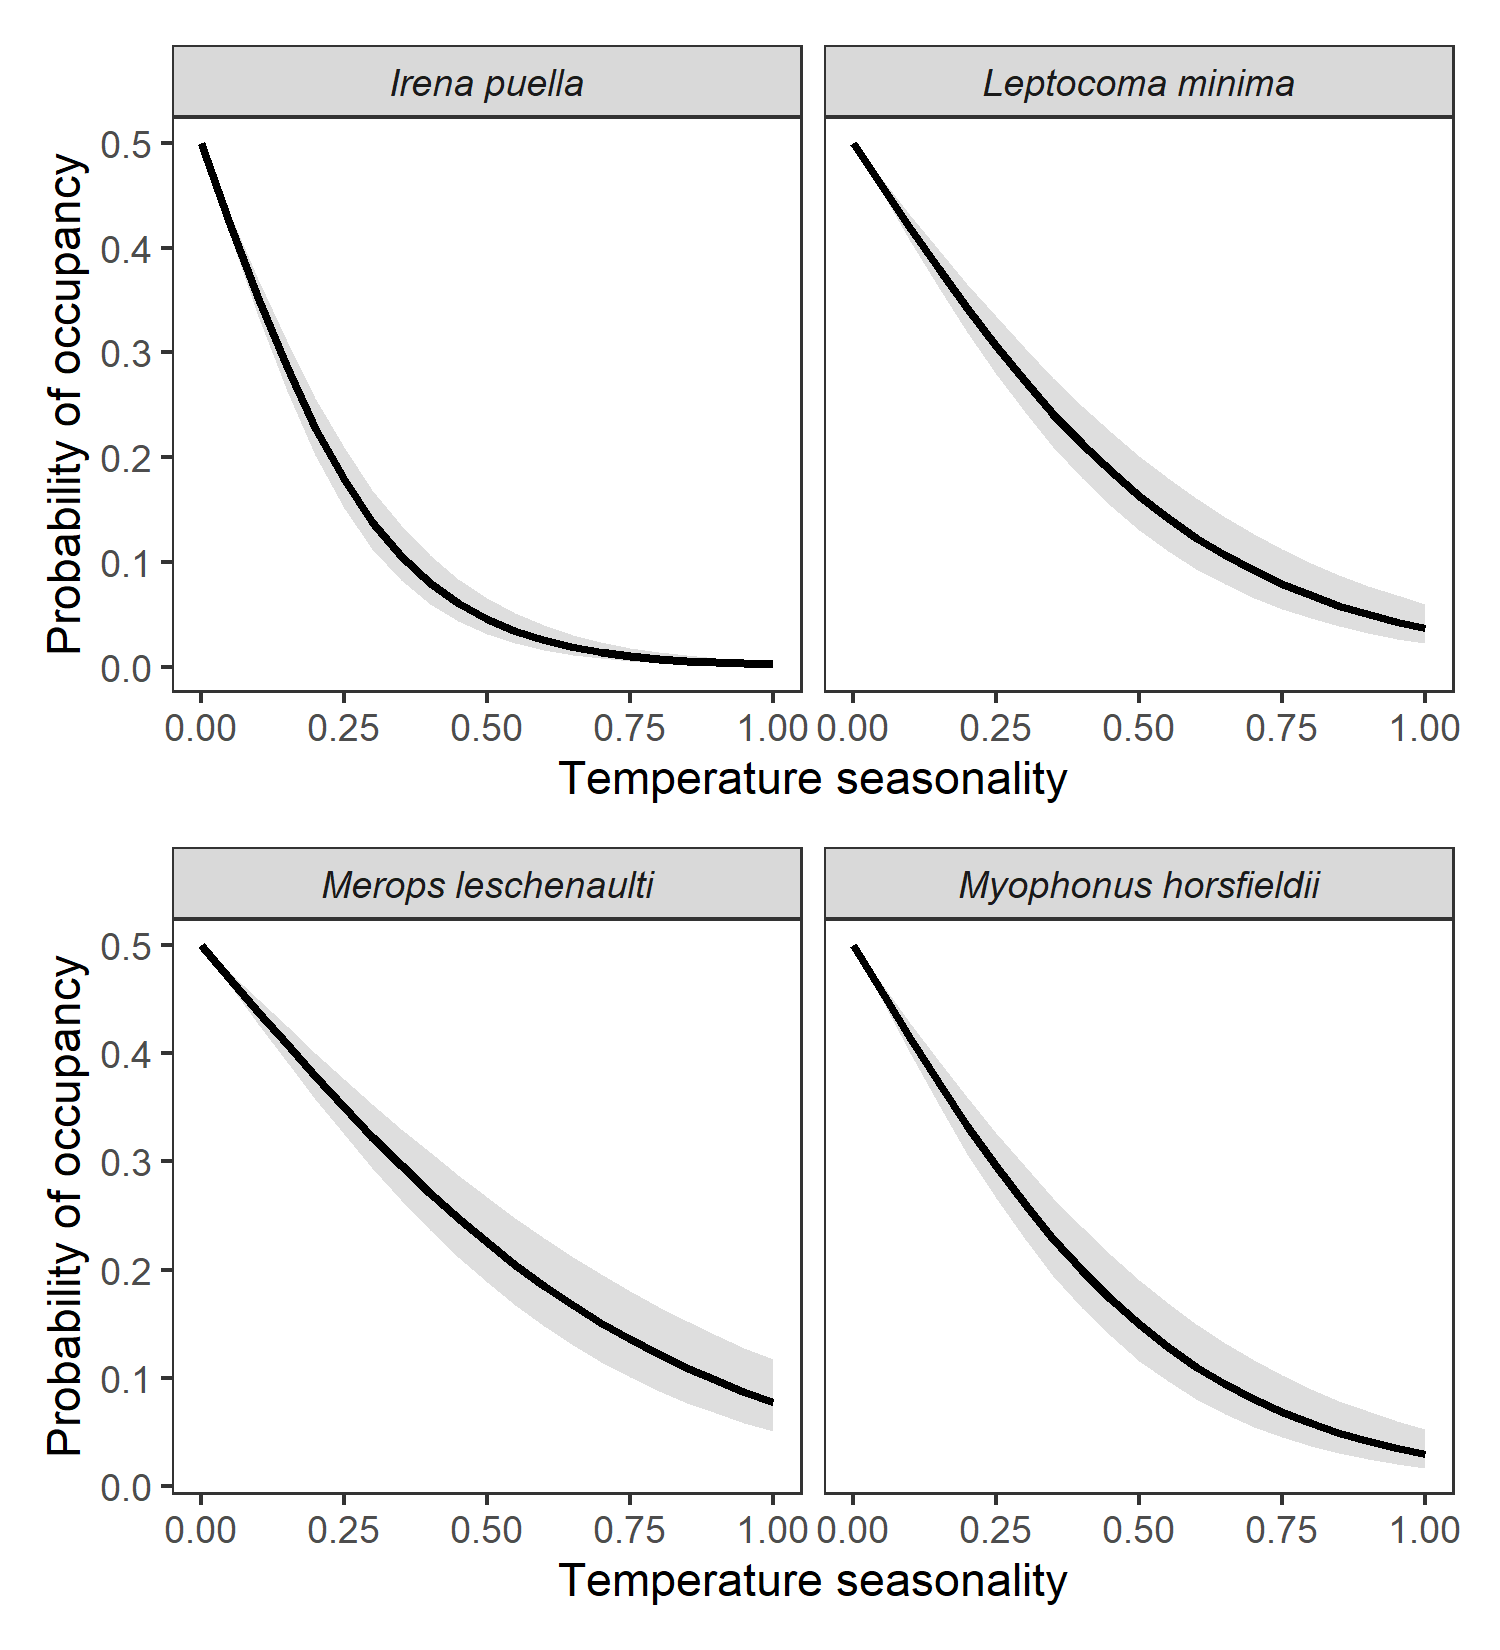
\includegraphics[width=0.9\textwidth]{figures/hillybirds/fig_05.png}
    \caption{
        \textbf{Probability of occupancy as a function of temperature seasonality.}
        Predicted probability of occupancy curves as a function of temperature seasonality for four forest species are shown here. 
        Temperature seasonality is negatively associated with the probability of occupancy of several forest species including the Asian fairy-blu\textit{eBird} (\textit{Irena puella}), the crimson-backed sunbird (\textit{Leptocoma minima}), the chestnut-headed bee-eater (\textit{Merops leschenaulti}) and the Malabar whistling-thrush (\textit{Myophonus horsfieldii}).
    }
    \label{hilly_fig_05}
\end{figure}

\begin{figure}[h!]
    \centering
    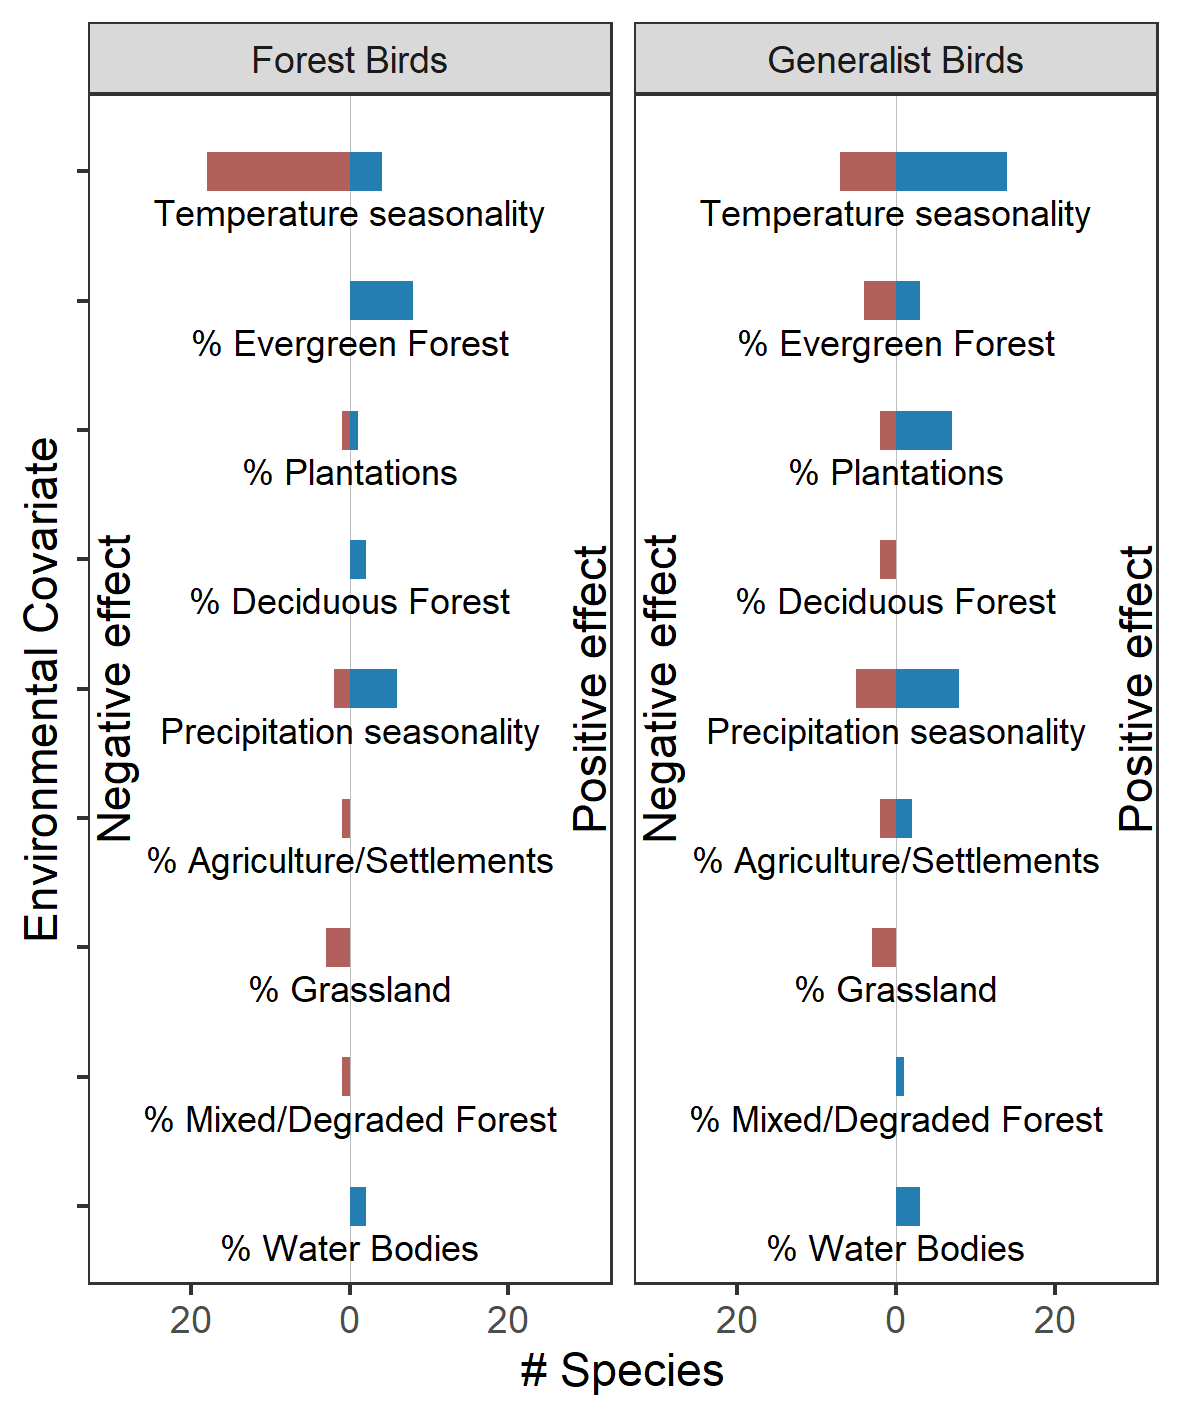
\includegraphics[width=0.9\textwidth]{figures/hillybirds/fig_04.png}
    \caption{
        \textbf{Environmental predictors and species-specific associations}.
        The direction of association between species-specific probability of occupancy and climatic and landscape predictors is shown here (as a function of habitat preference). 
        Blue colors show the number of species that are positively associated with a climatic/landscape predictor while red colors show the number of species that are negatively associated with a climatic or landscape predictor.
    }
    \label{hilly_fig_04}
\end{figure}

\subsubsection*{Bird-land cover associations}

Twenty-seven percent of species (n = 15 out of 55) were significantly associated with the proportion of evergreen forests.
Of these species, eight forest birds were positively associated.
Among generalist birds that showed a significant association with the proportion of evergreen forests, three species were positively associated while four were negatively associated.
A fewer number of species (n = 4) were significantly associated with the proportion of deciduous forests (positive association with two forest species and a negative association with two generalist bird species).
Six bird species showed a significant association with the proportion of grasslands.
Of these species, three forest bird species and three generalist birds showed a negative association (Fig.~\ref{hilly_fig_04}).
Five bird species were significantly and positively associated with the proportion of water bodies (n = 3 generalist birds and 2 forest birds).

\begin{figure}[h!]
    \centering
    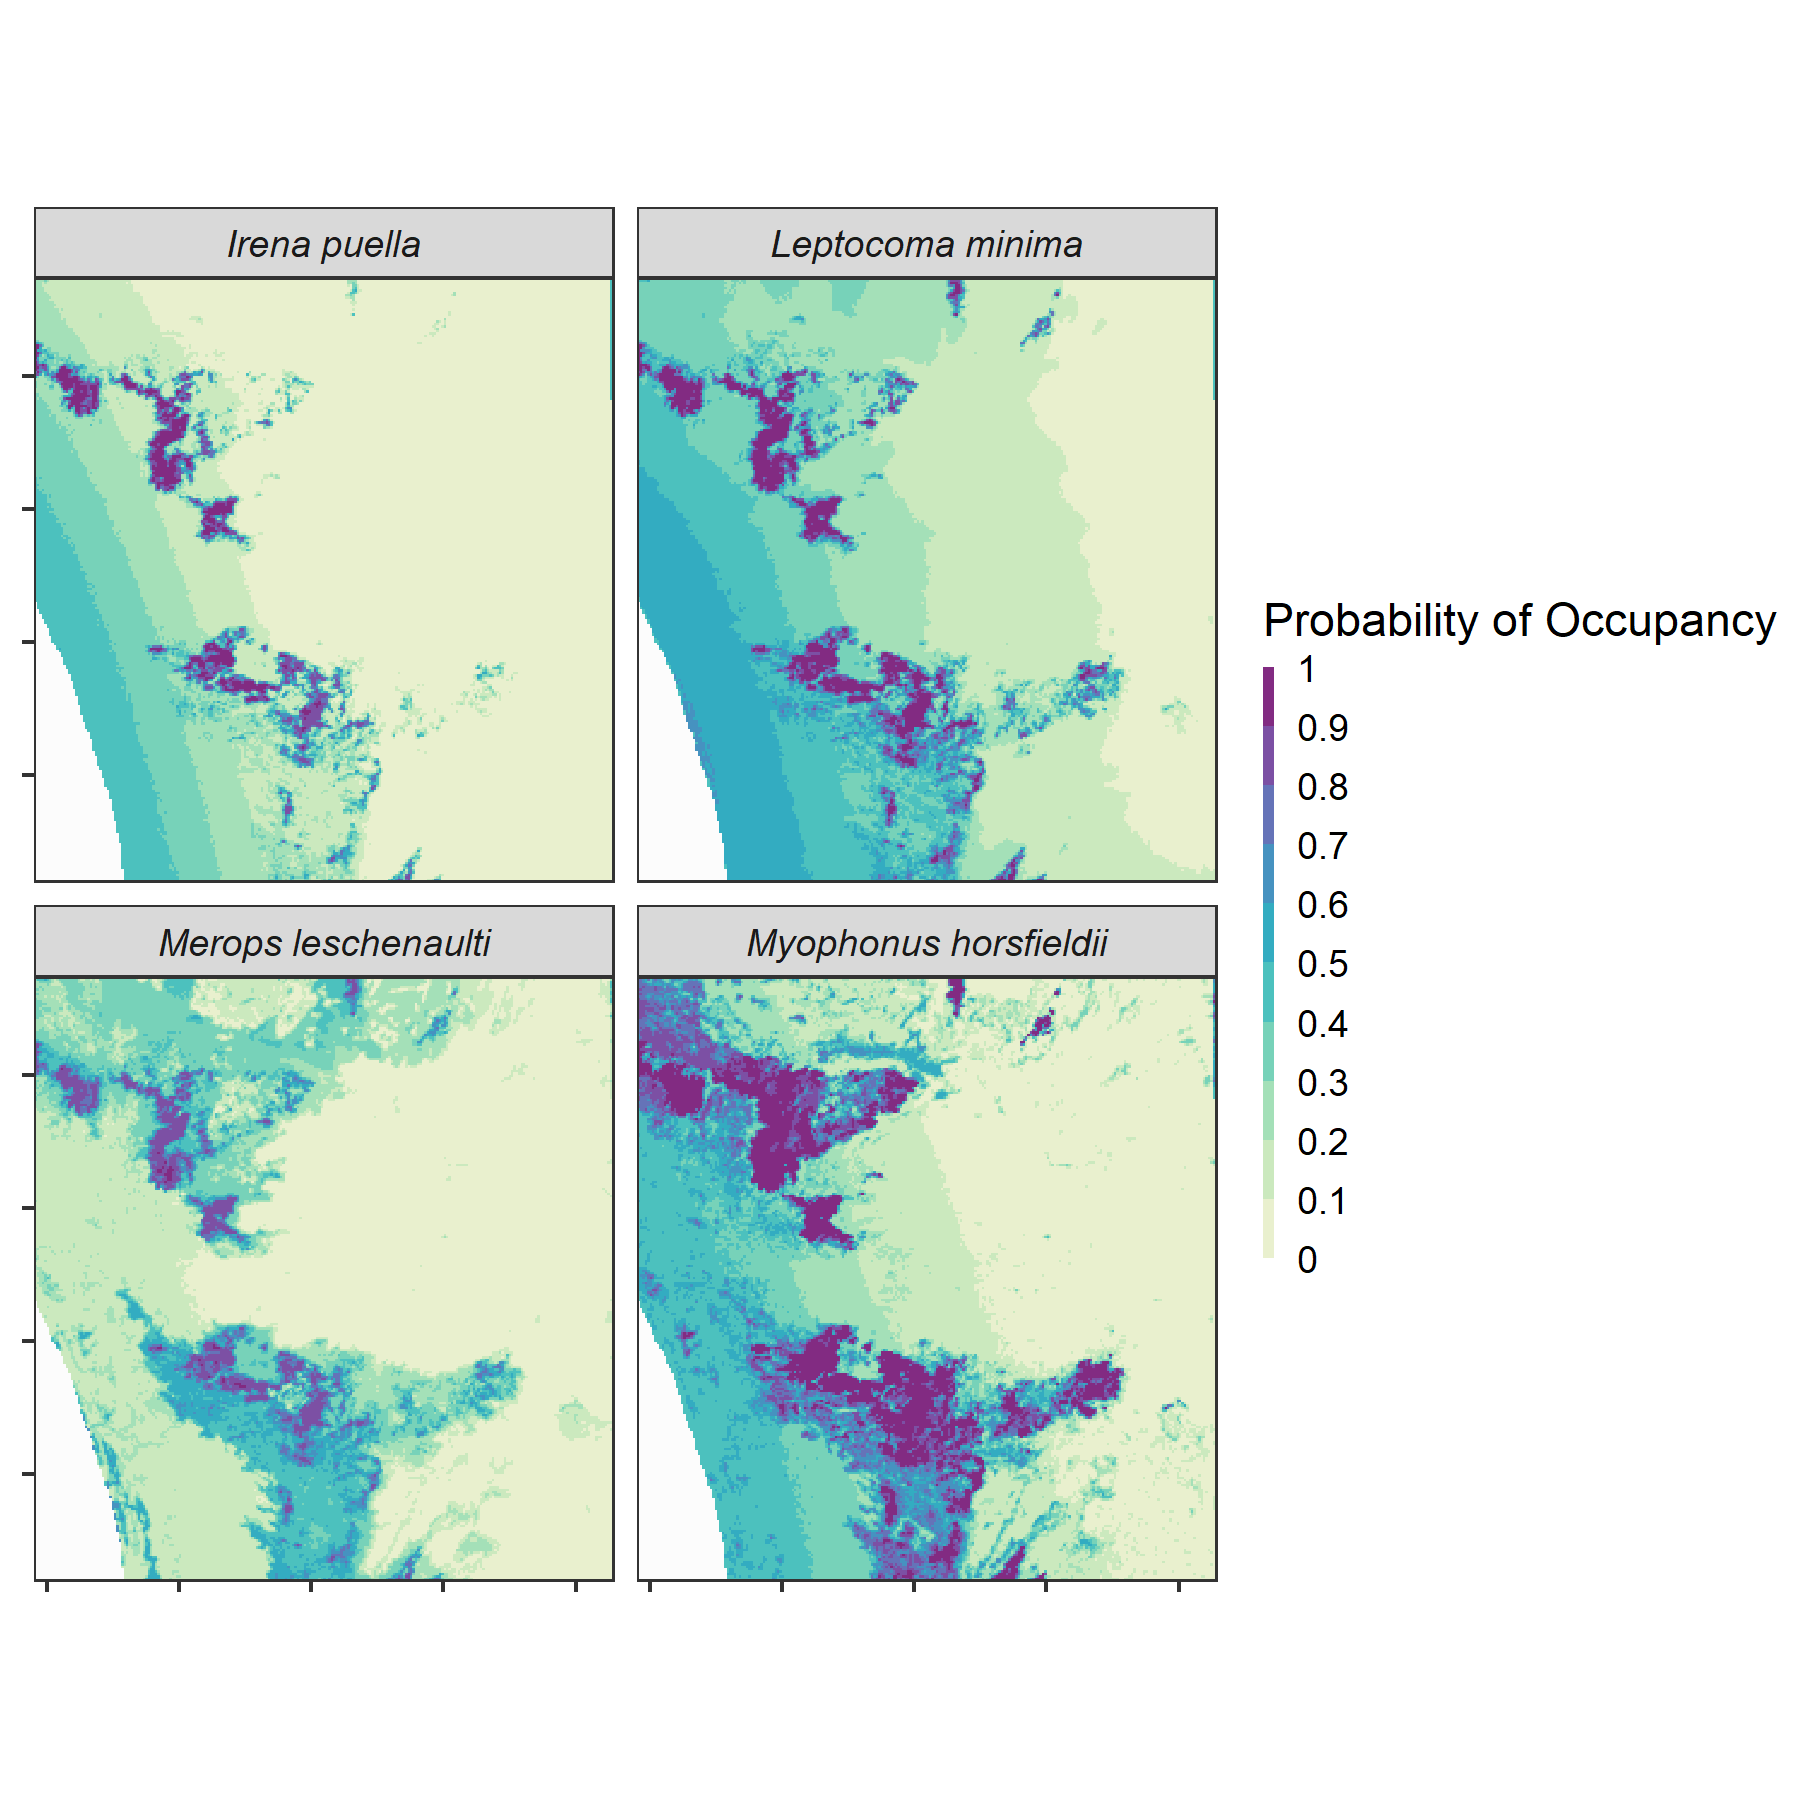
\includegraphics[width=0.9\textwidth]{figures/hillybirds/fig_06.png}
    \caption{
        \textbf{Predicted area of occurrence for four forest species.} 
        The probability of occupancy of the Asian fairy-blu\textit{eBird} (\textit{Irena puella}), the crimson-backed sunbird (\textit{Leptocoma minima}) and the chestnut-headed bee-eater (\textit{Merops leschenaulti}) is higher across the western slopes and at mid-elevations across our study area. The Malabar whistling-thrush (\textit{Myophonus horsfieldii}) has a higher probability of occupancy across mid-elevations throughout the study area examined.
    }
    \label{hilly_fig_06}
\end{figure}

33\% (n = 18 out of 55) of species examined were significantly associated with human-modified land cover types --- including the proportion of agriculture or settlements, plantations, and mixed or degraded forests.
One forest species showed a negative association, and one generalist species was positively associated with the proportion of mixed or degraded forests.
Five bird species showed a significant association with the proportion of agriculture or settlements.
Of these species, two generalist bird species showed a positive association while one forest species and two generalist bird species showed a negative association.

Eleven bird species showed a significant association with the proportion of plantations.
Of these species, one forest bird species showed a negative association, and one forest bird species showed a positive association.
Among generalist birds that showed a significant association with the proportion of plantations, seven birds were positively associated while two birds showed a negative association.

\section*{Discussion}

Our study shows that rigorously filtered and curated citizen science observations can be used within a robust statistical framework to inform our understanding of how environmental drivers are associated with species distributions.
We highlight the role of climate and land cover and its associations with bird occurrences along a tropical montane gradient in a biodiversity hotspot, the southern Western Ghats.

\subsubsection*{The role of temperature}

Tropical montane birds are especially vulnerable to ongoing changes in climate \citep{sekercioglu2007,perez2016,freeman2018,srinivasan2018}.
As a result of reduced temperature seasonality in the tropics relative to temperate regions, montane species in particular exhibit narrow thermal niches and hence, are likely to be unable to shift their distributions to track future climate changes \citep{janzen1967,deutsch2008,tewksbury2008,jankowski2013}.
Previous work in tropical areas across the globe have demonstrated that forest species are adapted to thermally aseasonal environments, while generalist species are more adapted to thermally variable, seasonal environments \citep{frishkoff2016,chan2016}.
In line with previous work, our study showed that several forest bird species (n = 18) were negatively associated with temperature seasonality.
Species such as the crimson-backed sunbird \textit{Leptocoma minima}, Asian fairy-blu\textit{eBird} \textit{Irena puella} and the chestnut-headed bee-eater \textit{Merops leschenaulti} for example showed a negative association (Fig.~\ref{hilly_fig_05}; Fig.~\ref{hilly_fig_06}).
The above result suggests that forest birds across the elevational gradient are potentially associated with narrow thermal niches.
Similar results have been demonstrated in the Western Himalayas, where birds occurring in forested habitats have narrow thermal niches relative to species in other land cover types \citep{srinivasan2019}.

In line with our hypothesis, the probability of occupancy of several generalist bird species (n = 14) was positively associated with temperature seasonality.
For example, the red-vented bulbul \textit{Pycnonotus cafer}, purple sunbird \textit{Cinnyris asiaticus}, and the spotted dove \textit{Streptopelia chinensis} showed a positive association.
Our result suggests that such generalist species occupy areas that show large variation in temperatures - including drier open habitats such as mixed or degraded forests and agricultural lands.
In fact, temperatures across tropical agricultural lands have been shown to be 7.6℃ higher than temperatures within tropical primary forests \citep{senior2017}.
Generalist bird species that showed a positive association likely possess broad thermal niches, relative to their forest counterparts.
However, our study also reported a negative relationship with temperature seasonality for seven generalist bird species, including the red-whiskered bulbul \textit{Pycnonotus jocosus} and the Oriental magpie-robin \textit{Copsychus saularis}.
Future studies need to consider climate-land cover interactions to explore patterns seen for generalist species.

\paragraph*{The role of precipitation}

The significant association with precipitation seasonality suggests the importance of the `hygric niche', which has been seldom explored empirically \citep{boyle2020}.
In other words, species' occupancy is often governed by a range of precipitation regimes which vary in turn by land cover type and topographic complexity \citep{nowakowski2018}.
Several forest and generalist species showed a positive association with precipitation seasonality.
Research from the Australian tropical rainforests suggests that precipitation seasonality was strongly associated with bird abundance \citep{williams2008}.
In addition, precipitation seasonality has been reported as a crucial factor influencing resource availability (e.g., insects) for bird populations \citep{loiselle1991}.
The positive association between precipitation seasonality and species occupancy (for forest and generalist birds) reported in this study can be explained by the cascading effect of rainfall on food availability and, thereby survival of birds \citep{butt2015,boyle2020}.
In our study, forest species such as the southern hill myna \textit{Gracula indica} and the crimson-backed sunbird \textit{Leptocoma minima}, and generalist species such as the rose-ringed parakeet \textit{Psittacula krameri} and the Indian white-eye \textit{Zosterops palpebrosus} showed a positive association.
On the other hand, we found that generalist species like the coppersmith barbet \textit{Psilopogon haemacephalus} and the red-vented bulbul \textit{Pycnonotus cafer} were negatively associated with precipitation seasonality.
Many of these generalist bird species that showed a negative association is associated with drier habitats across our study area.
Similar results have been reported from the neotropics where bird species largely associated with open habitats tend to prefer drier climates \citep{frishkoff2016}.
The above result merits further exploration that tests the interaction between precipitation seasonality and habitat structure and floristics in determining habitat use.
With increasing variability in rainfall patterns, it remains to be seen whether forest, as well as generalist bird species, adapt to such changes in the near future.
For instance, models have predicted reduced rainfall across regions in the Western Ghats as a result of future climatic changes \citep{rajendran2012}.

\subsubsection*{Role of naturally occurring vegetation and landscape transformation}

Apart from climate, certain land cover types are hypothesized to be crucial for many species, as they offer resources necessary for survival, breeding, and other activities \citep{sunarto2012}.
For insectivorous birds in central Jamaica, the landscape matrix and habitat type were vital in determining occupancy \citep{kennedy2011}.
Our study suggests a positive relationship for several forest species across naturally occurring land cover types --- evergreen and deciduous forests.
Few generalist species such as the Blyth's reed warbler \textit{Acrocephalus dumetorum} and gray wagtail \textit{Motacilla cinerea} were positively associated with the proportion of evergreen forests.
The above association can be attributed to the fact that the Blyth's reed warbler and the gray wagtail have been reported from forest edges as well as plantations and agricultural areas in the vicinity of evergreen forests.
It is also likely that our minimum spatial scale of 2.5km was coarse and resulted in sampling multiple land cover types.

As expected, several generalist bird species showed a positive association with human-modified land cover types.
This association highlights the role of habitat transformation.
The southern Western Ghats have undergone a drastic transformation in the last two decades, with the replacement of mid- and high-elevation forests and grasslands with exotic trees and plantations \citep{arasumani2018}.
In the Nilgiris alone, the area covered by exotic trees has almost doubled, from approx.
140 sq.km to 277 sq.km in the 44-year period between 1973 and 2017.
Generalist birds such as the jungle myna \textit{Acridotheres fuscus} and the red-whiskered bulbul \textit{Pycnonotus jocosus} were positively associated with the proportion of plantations.
On the other hand, we did see forest species like the Malabar whistling thrush \textit{Myophonus horsfieldii} showing a positive association with the proportion of plantations, which could be an artifact of this species often being reported in not only forested areas but forest edges and plantations as well.
In a complex matrix that is the Western Ghats, our results further lend support to the role of natural vegetation within these human-modified landscapes in sustaining biodiversity in the long term \citep{anand2010,ranganathan2010}.
For example, windbreaks, which are often thin slivers of natural vegetation present in tea plantations in our study area, have been shown to possess similar bird species richness compared to adjacent primary forests \citep{sreekar2013}.
In a similar vein, data from the Anamalai hills suggests that native shade trees within tea plantations bolster avian species richness almost two-fold compared to tea plantations without native shade trees \citep{raman2021}.
Furthermore, the type of human-modified land cover type matters too, and coffee, rubber, and areca plantations across the Western Ghats have been shown to support more bird species than tea plantations \citep{sidhu2010,karanth2016}.

\subsubsection*{Caveats and Conclusions}

Our analysis was carried out using semi-structured data derived from a large citizen science project.
The lack of experimental and sampling design of this study is a persistent criticism of citizen science research.
For example, a large proportion of checklists were reported within 200m of a road, which are relatively more accessible (Fig.~\ref{hilly_fig_03}a).
This pervasive spatial bias in sampling could impact results in ways that cannot be corrected via spatio-temporal filtering of data.
While citizen science observations are often seen as supplementary to (presumably) more rigorous, methodical sampling by trained observers, such sampling designs are often not logistically feasible at large spatial scales.
In under-studied or under-sampled regions, citizen scientists and their observations are first-class data sources with significant exploratory and explanatory power \citep{devictor2010,ellwood2017,robinson2020}.

Recent evidence also suggests that a species' response to environmental gradients or to drivers such as land cover and climate will vary as a function of biological traits \citep{mcgill2006}.
Our study classified species as forest species or generalist species \citep{ali1983}.
Other traits might better explain associations between climatic and land cover predictors and species' occupancy.
For example, body mass is often considered an indicator of thermoregulation, and has been shown to be strongly associated with thermal niches of species, particularly temperate species, and high elevation tropical species \citep{barve2021}.
Similarly, functional traits such as trophic niches, that explain dietary preferences of a particular species are often associated with the use of a particular habitat \citep{pigot2020}.
Himalayan birds --- which encounter a comparable, if wider, range of temperatures --- have been shown to use forest and agriculture habitats to cope with resource scarcity in winter, possibly indicating greater dietary generalization than previously thought \citep{elsen2018}.
Including functional traits is a promising avenue to better understand species' response to environmental change across human-modified landscapes in the Western Ghats, and tropical mountains more generally.

Over 60\% of mountainous landscapes across the planet are under tremendous anthropogenic pressures, and yet host some of the highest biodiversity in the world \citep{lasorte2010,elsen2020}.
The southern Western Ghats is one such human-dominated mountainous landscape, where understanding the role of climatic and landscape predictors in structuring species occupancy can inform conservation.
In this study, we show that species have differential responses to climate (temperature and precipitation) and natural and human-modified land cover types.
If species need to adapt to environmental changes, they need to be able to track their suitable climatic and habitat niche space, which may only be possible through the creation of climate corridors \citep{freeman2018}.

\newrefcontext[sorting=nyt]
\section*{Literature Cited}
\printbibliography[title=Literature~Cited,heading=none]
\end{refsection}
